\documentclass{article}
%\usepackage{maa-monthly}
\usepackage{college-math-j}
%% IF YOU HAVE FONTS INSTALLED
%\usepackage{mtpro2}
%\usepackage{mathtime}

%%
%% generated pictures separately from tikz files
%%
%\usepackage{tikz}
%\def\picdata=['#1', '#2']#3['#4', '#5']{\relax}
%\def\polydata=['#1', '#2']#3['#4', '#5']{\relax}
\usepackage{graphicx}

\newtheorem{theorem}{Theorem}
\newtheorem{conj}{Conjecture}
\theoremstyle{definition}
\newtheorem*{definition}{Definition}

\def\ZZ{\mathbb{Z}}
\def\pmod#1{(\bmod\  #1)}
\def\com#1{\quad\text{{#1}}\quad}
\def\ndiv{{\not|\;}}

\begin{document}

\title{On $\pmod{n}$ Spirals}
%\markright{Abbreviated Article Title}
\author{Andrew Reiter and Robin Young}

\maketitle

\begin{abstract}
  We introduce the concept of a $\pmod n$ spiral, and construct
  examples and visualizations of these.  A variety of patterns emerges
  and motivates the definition of a complete spiral.  We state and
  prove some interesting elementary facts about the existence of
  complete spirals.  We then introduce a number of generalizations and
  state related results.  The results and methods in the paper are
  elementary, and it is hoped that the accessibility of the material
  makes it suitable for discussion in high school mathematics classes.
  We have made our generation software freely available, and it is
  hoped that this paper and software will provide a resource to
  teachers and other interested parties in providing a tool for
  engaging the interest and participation of students, and/or for use
  in classroom learning to reinforce the process of observation,
  conjecture and proof.
\end{abstract}

\section{Spiral Construction}

We describe the construction of $\pmod{n}$ spirals and introduce the
notation we will use to analyze them.  These are similar in nature to
Ulam's Spiral \cite{Ulam}.  For a fixed integer $n \ge 2$, we will be
working with the additive group $\ZZ_n=\mathbb{Z}/n\mathbb{Z} = \{ 0,
1, \dots, n-1 \}$.  We begin with a square lattice $L$, which we can
take to be $\ZZ^2$.  Denoting the origin by $\ell_1 = (0,0)$, we build
the spiral by enumerating the lattice sites and assigning numbers from
$\mathbb{Z}_n$ in turn.  We spiral in a counter-clockwise direction
starting in the direction of the positive $x$-axis, so that $\ell_2 =
(1,0)$, $\ell_3 = (1,1)$, and the next four lattice points are $\{(0,
1),(-1, 1),(-1, 0),(-1, -1)\}$, respectively.  In general, once
$\ell_j$ has been assigned, and having chosen a `direction' by moving
from $\ell_{j-1}$, the next site $\ell_{j+1}$ is the site to the left
if this is not yet accounted for, or the site ahead otherwise.

Having enumerated the lattice as above, we now assign values from
$\ZZ_n$ as follows: to the origin we assign $\ell_1^* = 0$, and we then
count in $\ZZ_n$: $\ell_2^* = 1$, $\ell_3^* = 2$, etc., and cycling back to
$0$ after $n$ steps, so that $\ell_{n+1}^* = 0$. Continuing in this way,
we `count' all lattice sites $\pmod{n}$.  In general, this yields
\[
  \ell_j^* = j-1 \;\pmod n \quad\text{at site}\quad \ell_j.
\]
Figure~\ref{fig:squares} shows the $\pmod 8$ spiral construction in
three realizations: the first picture is the enumeration of lattice
sites, with successive squares shown; the second is the spiral
construction with the first complete spiral outlined; and the third is
the shaded realization of the $\pmod 8$ spiral, described below.  

\begin{figure}[htb]
  \centering
  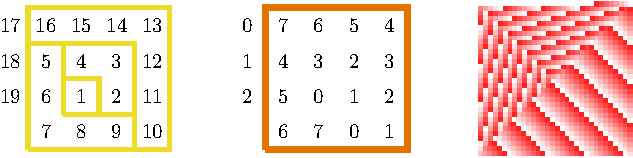
\includegraphics{Square.pdf}
  % \centering
  % \begin{minipage}{0.3\linewidth}
  %   \input pics/Square-1
  % \end{minipage}
  % \quad
  % \begin{minipage}{0.3\linewidth}
  %   \input pics/Square-2
  % \end{minipage}
  % \quad
  % \begin{minipage}{0.3\linewidth}
  %   \input pics/Square-3
  % \end{minipage}
  \caption{Construction of $\pmod 8$ spirals}
  \label{fig:squares}
\end{figure}

The first author's initial interest in generating spirals of
increasing size for various $\ZZ_n$ was to investigate some of the
patterns seen when using $\ZZ_{10}$ as the set of values.  In an
attempt to describe the patterns, he introduced the following
definition:

\begin{definition}%[complete spiral]
  A \emph{complete spiral} occurs when in the spiral construction, the
  partially completed spiral forms a square, and the last $\pmod{n}$
  value assigned is $\ell^*_i = n-1$, so all of $\ZZ_n$ has been used an
  integer number of times.
\end{definition}

We use the following notation: denote the first complete spiral
achieved by $Ond^1_n$; subsequent complete spirals are denoted
$Ond^k_n$, $k = 2,3,\dots$.  The number of times $\ZZ_n$ is used in
order to complete the $k^{th}$ square is called the iteration count.
The word ``ond'' is ``spiral'' in Swahili.

The first author generated several spirals with pencil and paper in a
methodical manner to create sets of complete spirals for various
values of $n$ and $k$.  While tedious and not exactly related to the
initial goal of looking at diagonal patterns, he realized that there
seemed to be patterns found in the construction of the spirals.
Specifically, there were patterns in the sizes of the complete
spirals, iteration counts, and where the last lattice point rested;
this led the author to investigate what these patterns were.

\subsection{On the side lengths and iterate counts of $Ond^k_n$}

In order to investigate these patterns, the author determined that
more data was needed and, due to the tedium of pencil and paper, a
program should be written to generate complete spirals
\cite{PySquare}.  This allowed the author to generate a larger number
of complete spirals and collect data on lengths, iterations, and
ending points.

In analyzing the data, for small choices of $n$ and $k$, a few
recurring patterns were found: specifically, denoting the side length
and iteration count of $Ond^k_n$ by $\lambda$ and $\xi$, respectively,
several formulae for the tuple $(\lambda,\xi)$ were observed,
including $(kn, k^2 n)$, $(\frac{kn}{2}, \frac{k^2 n}{4})$, and
$(\sqrt{n}k, k^2)$.  To further understand these patterns, the prime
factorization of $n$ for each complete spiral $Ond^k_n$ with the
lengths and iteration data was generated for analysis.  From this
data, the first author determined there was a relation involved with
finding the greatest square divisor of $n$, which led him to
conjecture the following:

\begin{theorem}%[Length of Sides of $Ond^k_n$]
\label{lenthm}
Let $s$ denote the greatest square divisor of $n$.
The complete spiral $Ond^k_n$ has the following structure:
\begin{itemize}
\item If $\lambda$ is the length of the sides of $Ond^k_n$, then
\begin{equation}
  \lambda = \frac{kn}{\sqrt{s}}.
\label{lambda}
\end{equation}
\item If $\xi$ is the iteration count of $Ond^k_n$, then
\begin{equation}
  \xi = \frac{k^2n}{s}.  
\label{xi}
\end{equation}
\item If $\ell_{max} \in L$ is the last lattice point in the complete
  spiral $Ond^k_n$, then $\ell_{max}$ is either the top-right corner or
  bottom-left corner of the square.  If both $n$ and $k$ are odd, then
  $\ell_{max}$ will be the top-right corner of $Ond^k_n$.  In all other
  cases, $\ell_{max}$ will be the bottom-left corner.
\end{itemize}
\end{theorem}

One will note that in the case where $n$ is square-free, then $s=1$
and \eqref{lambda} and \eqref{xi} reduce to $\lambda = k n$ and $\xi =
k^2 n$, respectively.  These can be considered a worst case, in that
the only complete spirals are those whose side lengths are a multiple
of $n$.  One might also consider these to be the least robust in the
case of length and iteration counts.

An interesting and surprising aspect to this process of complete
spiral construction is the connection to the greatest square divisor
of the integer $n$.  To see this more clearly, choose some $n$ and
construct, by hand, the spiral $Ond^1_n$.  At this point, you know
$\lambda$ and $\xi$, so pick one, substitute $k = 1$ and solve for
$s$.  This yields a geometric and constructive (albeit impractical)
approach to finding the greatest square divisor of a number.

In the process of investigating sizes and iteration counts of
$Ond^k_n$, the first author implemented a method to map the generated
spirals to grayscale images. This works best for positive integers,
$n$, less than 256.  The map $f : \ZZ_n \to \ZZ_{256}$ is defined by a
scaled floor function,
\begin{equation}
   f(j) = \alpha j, \quad \text{where} \quad
   \alpha = \left\lfloor \frac{255}n \right\rfloor.
\label{grayscale}
\end{equation}
The function $f$ thus maps $\ZZ_n$ to a set of brightness values which
are used to generate grayscale images.  This is seen in the third
picture of Figure~\ref{fig:squares}, and again in Figure~\ref{fig:bigsquares}.

\begin{figure}[htb]
  \centering
  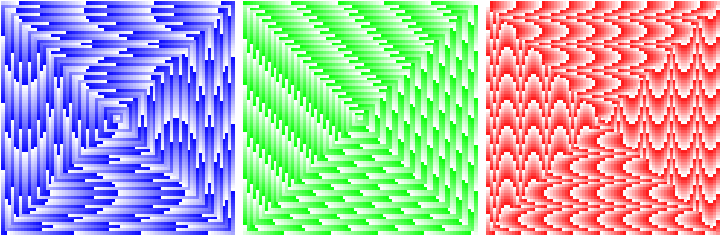
\includegraphics{Sqr}
  % \centering
  % \begin{minipage}{0.3\linewidth}
  %   \input pics/Sqr-1
  % \end{minipage}
  % \quad
  % \begin{minipage}{0.3\linewidth}
  %   \input pics/Sqr-2
  % \end{minipage}
  % \quad
  % \begin{minipage}{0.3\linewidth}
  %   \input pics/Sqr-3
  % \end{minipage}
  \caption{Square spirals, $\pmod{23}$, $\pmod{16}$ and $\pmod{9}$.}
  \label{fig:bigsquares}
\end{figure}

In Figure~\ref{fig:bigsquares}, we see a few of the patterns that
emerge as the value of $n$ changes.  The figures are $80\times80$
spirals, counted  $\pmod{23}$, $\pmod{16}$ and $\pmod{9}$,
respectively.  The most regular pattern is seen when $n=16$, and the
and the most complicated of these is $n=23$.  In each
picture there is a noticeable repeating pattern, and these in turn seem
to scale approximately uniformly.

\begin{proof}[Proof of the Theorem]
  Recall that $n\ge 2$ is fixed.  Let $\lambda$ be the length of the
  side of a complete spiral, and let $\xi$ be the corresponding
  iteration count.  Since the spiral is square, we must have $\xi n =
  \lambda^2$, and so $n \mid  \lambda^2$.  Now any prime which divides
  $n$ must also divide $\lambda^2$, and must thus divide $\lambda$.

  Since $s$ is the greatest square divisor of $n$, we can uniquely
  write $n = q^2_1\, q_2$, where $q_1^2 = s$ and $q_2$ is square-free.
  It follows that $q_1^2\mid \lambda^2$, so $q_1\mid \lambda$.  We can thus
  divide by $q_1^2$, and we obtain $q_2 \mid  ({\lambda}/{q_1})^2$.  Since
  $q_2$ is square-free, we have $q_2\mid  ({\lambda}/{q_1})$, so we must
  have $\lambda = k \,q_1 \,q_2$ for some integer $k$; it is also
  clear that $n\mid \lambda^2$ for any such $\lambda$.  We conclude
  that $\lambda = k \,q_1\, q_2$ is the side of the $k$-th complete
  spiral $Ond^k_n$, $k = 1,2,\dots$.

  Equation \eqref{lambda} now follows since $\sqrt{s} = q_1$, and
  \eqref{xi} follows since $\xi = \frac{\lambda^2}{n}$.  The final
  claim follows since $\ell_{max} = \lambda^2$ is even unless $k$, $q_1$
  and $q_2$ are all odd, and by construction $\ell_{max}$ represents the
  top-right corner of the square if it is odd, and the bottom-left
  corner if it is even.
\end{proof}

\section{Generalizations to higher dimensions}

The second author proposed investigating the idea how of $Ond$ might
work for cubes or higher dimensional squares, since the lattice is the
basis for the spiral. In imagining dimensions $d = 3$ and $d=4$,
finding routes in the lattice to enumerate the spiral, either in $\ZZ$
or in $\ZZ_n$, becomes an interesting task; an algorithm and a method
for visualizing these would also be challenging.

In terms of planar spirals described above, we are interested in
finding squares, which led to the areal requirement $n\mid \lambda^2$. For
cubic spirals, we would have the corresponding volume requirement
$n\mid \lambda^3$, and similarly for 4- or $d$-dimensional hypercubic
lattices, we would require $n\mid \lambda^4$ or $n\mid \lambda^d$,
respectively.  Thus we can generalize the cubic spirals $Ond_n$ for
any dimension $d$, using the analogous $d$-dimensional volume
requirement, without having to visualize the hypercubes.

\begin{theorem}
\label{dimdthm}
Suppose $n\mid \lambda^d$ for some $d\ge 2$, and write $n$ as $n=q\,m^d$,
where $m \in \mathbb{N}$ and $q$ is $d$-th power free.  If $q$ has the
(unique) prime decomposition
\[
  q = \prod_{j=1}^{r} p_j^{e_j}, \com{with each}
  0<e_j<d,
\]
then $\lambda$ must have the form
\[
  \lambda = k \,m\, \textstyle{\prod}\, p_j, \com{for some}
  k \ge 1.
\]
\end{theorem}

\begin{proof}
The proof is analogous to that of Theorem~\ref{lenthm}.
Since $n\mid \lambda^d$, we have 
\[
  m^d\mid \lambda^d   \com{so that}
  m\mid \lambda ,
\]
and $\lambda/m$ is an integer.  Thus we can write $q\mid (\lambda/m)^d$,
and so also $p_j\mid (\lambda/m)^d$ for each $j$.  Since $p_j$ is prime,
we have $p_j\mid (\lambda/m)$, and this holds for each distinct prime
$p_j$.  It follows that $\prod p_j\mid (\lambda/m)$, and we can write
\[
  \lambda = k\, m\, \textstyle{\prod}\, p_j  \com{for some} k.
\]
For any such $\lambda$, it is immediate that $n=q\,m^d$ divides
$\lambda^d$, completing the proof.
\end{proof}

\section{Other Planar Shapes}

An alternative generalization is to remain in the plane, while
considering other lattice structures in the plane.  We again enumerate
the lattice by spiraling out from the origin, and form the complete
lattices by counting in $\ZZ_n$ and by declaring a complete spiral in
the same way: that is, an $Ond$ is achieved when the scaled shape is
achieved by assigning $n-1$ to the last site in that shape.

\subsection{Triangular Spirals}

Recall that the triangular numbers count the area of successive
lattice triangles \cite{OEIS}, and are given by
\[
  T_m = Area(\triangle m) = 1+2+\dots+m = \frac{m(m+1)}2,
\]
and these are visualized and enumerated in
Figure~\ref{fig:triangles}.  Here we have enumerated in a
counter-clockwise direction, and have staggered the lattice to retain
symmetry: thus the first five lattice points are
\[\textstyle{
  \ell_1 = (0,0), \quad
  \ell_2 = (1,0), \quad
  \ell_3 = (\frac12,\frac{\sqrt3}2), \quad
  \ell_4 = (0,\sqrt3), \quad
  \ell_5 = (-\frac12,\frac{\sqrt3}2).}
\]
On the left we have enumerated the lattice, in the center we have
counted $\pmod 3$, and on the right we have counted $\pmod 5$.  and
shown the first few complete spirals.  The yellow lines outline all
possible triangles, and the orange lines outline complete spirals.

\begin{figure}[htb]
  \centering
  \includegraphics{Triangle.pdf}
  % \centering
  % \begin{minipage}{0.3\linewidth}
  %   \input pics/Tri-1
  % \end{minipage}
  % \quad
  % \begin{minipage}{0.3\linewidth}
  %   \input pics/Tri-2
  % \end{minipage}
  % \quad
  % \begin{minipage}{0.3\linewidth}
  %   \input pics/Tri-3
  % \end{minipage}
  \caption{Triangular spirals: enumerated and counted $\pmod 3$ and
    $\pmod 5$.}
  \label{fig:triangles}
\end{figure}

Proceeding as above, we see that we have a complete $Ond_n$ spiral
when $n\mid T_m$, that is, when $n\mid \frac{m(m+1)}2$.  Due to the factors
$m$ and $m+1$, it is reasonable to check when $n\mid T_m$ and also either
$n\mid T_{m-1}$ or $n\mid T_{m+1}$, that is, we have consecutive pairs of
complete triangular spirals.  To begin checking this, we generate the
values
\[
  \{ T_m \} =
  \{ 1, 3, 6, 10, 15, 21, 28, 36, 45, 55, 66, 78,
     91, 105, 120, 136, \dots \}
\]
and observe when $n\mid T_m$, for fixed small values of $n \ge 2$.

It is clear that only the even valued $T_m$ are $Ond_2$ achievable,
the first several such being
\[
T_3,\ T_4,\ T_7,\ T_8,\ T_{11},\ T_{12},\ T_{15},\ T_{16},\  T_{19},\ T_{20}.
\]
From this limited sample, it looks like complete $Ond_2$ spirals always
appear in pairs.  The same observation holds for each of
$n = 3,\ 4,\ 5,\ 7,\ 8,\ 9,\ 11,\ 13,\ 16$.
However, the spiral $Ond_6$ is achieved by
\[
T_3,\ T_8,\ T_{11},\ T_{12},\ T_{15},\ T_{20},\ T_{23},\ T_{24},\ \ldots,
\]
so that, although some complete spirals are achieved by consecutive
triangles, there are also isolated complete spirals.  Similar
observations follow for $n=10$, $12$, $14$ and $15$.

More generally, suppose that $n\mid T_{m-1}$ and $n\mid T_m$, so that
consecutive complete triangular spirals $Ond_n$ are achieved.  Then
$n$ also divides the difference
\[
  T_m - T_{m-1} = \frac{m(m+1)}2 - \frac{(m-1)m}2
     = m,
\]
and we have consecutive $Ond_n$s in the pair $\{T_{m-1},\ T_m\}$
provided
\[
  n\mid m \com{and} 2n\mid 2T_m=m(m+1),
\]
Also, since $n$ cannot divide both $m$ and $m+1$,
complete triangular spirals can never occur in consecutive triples
$\{T_{m-1},\ T_m,\ T_{m+1}\}$.

It follows that for any $n$, by taking $m=2\,k\,n$, say, we always
achieve some consecutive spirals.  We can also ask for which values of
$n$ we \emph{always} have spiral pairs, that is, there are no isolated
spirals.  A complete spiral is isolated if we have
\[
  n \mid T_m=\frac{m(m+1)}2 \com{while also}
  n \ndiv m, \quad  n \ndiv m+1.
\]
This can occur if $n$ has different factors, some of which divide $m$
and some dividing $m+1$.  In particular, if $n$ is a power of a single
prime, this cannot happen.

\begin{theorem}
\label{thm:tri}
If $n$ is a prime power, then complete $Ond_n$ spirals
always appear in consecutive pairs; if not, there are always isolated
complete $Ond_n$ spirals.
\end{theorem}

\begin{proof}
First we take $n=p^r$ where $p$ is prime, and suppose that
\[
  p^r = n\mid T_m=\frac{m(m+1)}2,
\]
so $T_m$ is a complete spiral.  Then either $p\mid m$ or $p\mid m+1$, but not
both.  In either case, since $p$ is prime, we have $n=p^r\mid m$ or
$n=p^r\mid m+1$, so that
\[
  n\mid T_m - m = T_{m-1}  \com{or}
  n\mid T_m + m+1 = T_{m+1},
\]
respectively, and $T_m$ is part of a consecutive complete spiral pair.

Next, suppose that $n$ is a composite number, with at least two
distinct prime factors.  We must exhibit a value of $m$ such that
$n\mid T_m$, that is $2n\mid m(m+1)$, but $n$ does not divide either $m$ or
$m+1$.  Since $n$ has at least two distinct prime factors, we can
write $2\,n = s\,t$, where $s$ and $t$ have no common factors, and
there are distinct prime factors $p$ and $q$ of $n$, with $p\mid s$ and
$q\mid t$.

We use the well-known fact \cite{Davenport} that for coprime $s$
and $t$, there exist integers $a$ and $b$ such that
\begin{equation}
  a\,s + b\,t = 1.
\label{Bezout}
\end{equation}
It is clear that (only) one of $a$ and $b$ must be negative, say
$b<0$.  Then we set
\[
  m = -b\,t>0, \com{so also}
  m+1 = a\,s.
\]
With this choice of $m$, we have
\[
  m(m+1) = -b\,t\,a\,s = -2\,a\,b\,n, \com{so that}
  n\mid T_m.
\]
On the other hand, we have $p\mid s$, so $p \ndiv {-bt}$ (because $p\mid {-bt}$
would contradict \eqref{Bezout}), so that $p \ndiv m$, and similarly
$q\mid t$ so $q \ndiv as=m+1$.  Since $p$ and $q$ are both factors of
$n$, it follows that $n$ does not divide either $m$ or $m+1$, and so
$T_m$ is an isolated complete $Ond_n$ spiral.
\end{proof}

There are infinitely many different solutions of \eqref{Bezout}, for
each distinct decomposition $2\,n=s\,t$; each such solution gives an
isolated complete spiral.  Also, as we have seen, $\{T_{m-1},T_m\}$
gives a complete spiral pair for any $m=k\,n$ if $n$ is odd, or
$m=2\,k\,n$ if $n$ is even.  Note that if $n$ is even, and $m$ is an
odd power of $n$, then $T_m$ is not a complete spiral: indeed, $m+1$
is odd, and so one power of 2 is canceled in forming $T_m$, so that
$n \ndiv T_m$ in this case.

\begin{figure}[htb]
  \centering
  \includegraphics{Tri.pdf}
  % \centering
  % \begin{minipage}{0.3\linewidth}
  %   \input pics/Tri-S
  % \end{minipage}
  % \quad
  % \begin{minipage}{0.3\linewidth}
  %   \input pics/Tri-T
  % \end{minipage}
  % \quad
  % \begin{minipage}{0.3\linewidth}
  %   \input pics/Tri-H
  % \end{minipage}
  \caption{Visualization of triangular spirals}
  \label{fig:trishades}
\end{figure}

As with the square spirals above, we visualize larger triangular
spirals by grayscale images, using the grayscale map $f$ defined in
\eqref{grayscale}.  Coloring rectangles as in the previous case gives an
angular picture in which the symmetry is slightly obscured, so we try
some alternative shapes.  It is natural to use triangles, which mimic
the shape of the spiral, but while these respect the symmetry of the
triangle, they do not fill out the whole plane, so patterns are harder
to recognize.  Instead, we use hexagonal cells to visualize the
spirals: these respect the symmetry and fill out the plane, and are
the cleanest visually.  This is not unexpected, as the hexagonal
lattice is the lattice dual of the triangular lattice with which we
are working.  In Figure~\ref{fig:trishades} we show three such
visualizations of the same triangular spiral, respectively shaded with
rectangular, triangular and hexagonal cells.  We show the complete
spiral with 496 points and with $k=8$: this is $Ond_8^3$.

\subsection{Hexagonal Spirals}

Using the same lattice points as used for the triangular lattice, we
can also spiral out from the origin in an hexagonal pattern.  Again we
spiral in a counter-clockwise direction, enumerating the cells,
counting in $\ZZ_n$, or visualizing them as in the earlier cases.  The
enumeration, $\ZZ_7$ counting and grayscale visualizations are shown
in Figure~\ref{fig:hex}; in addition, all hexagons are outlined in the
first picture, and the first complete $Ond_7$ spiral is outlined in
the second.  As with the triangular spiral, the grayscale
visualization is cleanest when using hexagonal cells.

\begin{figure}[htb]
  \centering
  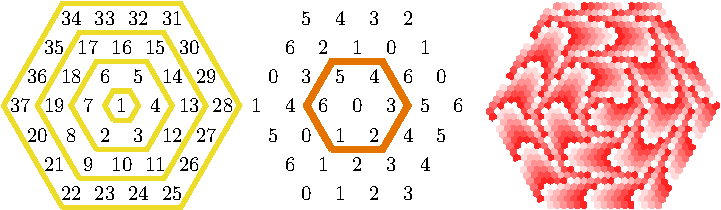
\includegraphics{Hexagon.pdf}
  % \centering
  % \begin{minipage}{0.3\linewidth}
  %   \input pics/Hexagon-1
  % \end{minipage}
  % \quad
  % \begin{minipage}{0.3\linewidth}
  %   \input pics/Hexagon-2
  % \end{minipage}
  % \quad
  % \begin{minipage}{0.3\linewidth}
  %   \input pics/Hexagon-3
  % \end{minipage}
  \caption{Hexagonal spirals: enumerated, $\pmod 7$ and grayscale}
  \label{fig:hex}
\end{figure}

In enumerating the hexagonal spiral, some observations are immediate:
the first is that the successive hexagons are concentric, unlike the
previous cases.  We can use this observation to count the spiral:
these are the centered hexagonal numbers \cite{OEIS}.  The innermost hexagon has
one element, and successive hexagons contribute a multiple of 6 to the
total: thus the first few numbers are
\[
  1,\quad 1+6=7,\quad 7+2\cdot6=19,\quad 19+3\cdot6=37, \com{etc.,}
\]
and in general we deduce that
\begin{align*}
  CH_m &= 1 + 6\,(1 + 2 + \dots + (m-1) ) \\
       &= 1 + 6\,T_{m-1} = 1 + 6\,\textstyle{\frac{(m-1)m}2},
\end{align*}
these consisting of the set
\[
  \{CH_m\} = \{ 1,\ 7,\ 19,\ 37,\ 61,\ 91,\ 
        127,\ 169,\ 217,\ 271,\ldots \}.
\]

Because $CH_m = 1+6\,r$, it follows that any number $n$ with 2 or 3 as
a factor cannot support $Ond_n$.  That is, any number $n$ which has
complete spirals must be of the form
\[
  n = 1 \pmod 6  \com{or}  n = -1 \pmod 6.
\]
The effect of different $n$ is seen in Figure~\ref{fig:hexN}: we show
the $\pmod n$ spirals for $n=5$, 6 and 7, respectively, with the
complete $Ond_7$ spirals outlined.  The uniformity in the $\pmod6$
spiral reflects the fact that $CH_m=1\pmod6$ for all $m$.

\begin{figure}[htb]
  \centering
  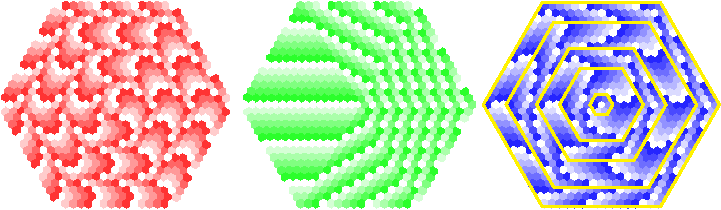
\includegraphics{Hex-n.pdf}
  % \centering
  % \begin{minipage}{0.3\linewidth}
  %   \input pics/Hex-5
  % \end{minipage}
  % \quad
  % \begin{minipage}{0.3\linewidth}
  %   \input pics/Hex-6
  % \end{minipage}
  % \quad
  % \begin{minipage}{0.3\linewidth}
  %   \input pics/Hex-7
  % \end{minipage}
  \caption{Hexagonal $\pmod5$, $\pmod6$ and $\pmod 7$ spirals}
  \label{fig:hexN}
\end{figure}

Our investigations indicate that any such $n$ has only prime factors
of the form $p=6\,q+1$.  Moreover, any $n$ which is a product of
primes $p=6\,q+1$ appears to support complete hexagonal spirals
$Ond_n$.  We state this as a conjecture:

\begin{conj}
  Complete hexagonal spirals are $Ond_n$ achievable if and only if $n$
  is a product of primes of the form $p=6\,q+1$.
\end{conj}

\begin{proof}[Discussion]
We can prove the ``only if'' part, which states that any prime $p$
such that $p\mid CH_m$ has the form $p=1\pmod6$, as follows.

Write $CH_m = 3m^2+3m+1$, and suppose $p\mid CH_m$.  Then also
\[
  12\,p\mid 36m^2+36m+12 = 9(4m^2+4m+1)+3 = [3(2m+1)]^2+3,
\]
so that $[3(2m+1)]^2 = -3 \pmod p$.  We now invoke the law of
quadratic reciprocity \cite{Davenport}, which in this case states that $-3$ is
a square $\pmod p$ if and only if $p$ is a square $\pmod 3$.  Since
the only squares $\pmod 3$ are 0 and 1, and $3\ndiv p$, we must have
$p=1\pmod 3$.  Since $p$ is also odd, it follows that $p=1\pmod 6$, as
required.

To verify the other half of the conjecture, we would need to exhibit
an $m$ such that $n\mid CH_m$ for any $n$ which is a product of primes
of the form $p=1\pmod 6$.  Write $CH_m = 1 + 6\,T_{m-1}$, and suppose
$n$ is a product of primes which are $1\pmod6$.  Then also $n=6r+1$,
and $n\mid CH_m$ is
\[
  1 + 6\,T_{m-1} = a\,(6\,r+1) = 6\,a\,r + a,
\]
so that $a = 1\pmod 6$, which is $a=6\,t+1$.  Plugging in and
simplifying, this becomes
\[
  T_{m-1} = 6\,t\,r + t + r = n\,t + r,
\]
or equivalently
\begin{equation}
  T_{m-1} = r \pmod {6r+1} = r \pmod n.
  \label{Tmqp}
\end{equation}

Next, we note the identities
\[
  T_{j+n} - T_j = \frac{n(n+1+2j)}2  \com{and}
  T_{n-1-j} - T_j = \frac{n(n-1-2m)}2,
\]
which hold for all $n$ and $j$, and in particular, if $n$ is odd, then
for any $j$,
\[
  T_{j+n} = T_j\pmod n \com{and}  T_{n-1-j} = T_j\pmod n.
\]
By subtracting multiples of $n$ and applying the second identity, it
follows that \eqref{Tmqp} has a solution if and only if it has a 
solution with $1\le m\le \frac{n-1}2 = 3\,r$.
\end{proof}

In light of this discussion, Conjecture 1 is equivalent to the
following alternative conjecture, which we have computationally
validated for all values of $n$ up to one million.

\begin{conj}
For any $r\ge 0$ such that $n=6\,r+1$ has only factors of the form
$p=1\pmod6$, the equation
\[
  T_{m-1} = r\pmod n = r \pmod{6\,r+1}
\]
has a solution with $1\le m\le 3\,r$.
\end{conj}


\section{Further Areas of Investigation}

There are essentially two steps in our basic pattern constructions:
the first is to form the spiral, and the second is to count it in
$\ZZ_n$.  The square, triangular and hexagonal spirals discussed above
are the only spirals that can be formed out of a regular tiling of the
plane.  We identify the candidates for complete $Ond_n$ spirals as
$S_m = F_S(m)$, these being the square, triangular or centered hexagonal
numbers, and our condition for a complete spiral is then
\[
  n \mid S_m = F_S(m).
\]
This is an abstract condition and we could pose the general problem
as, given some increasing function $F:\ZZ_+\to\ZZ_+$ and some integer
$n$, identify the values $m$ for which we have $n\mid F(m)$.

\begin{figure}[htb]
  \centering
  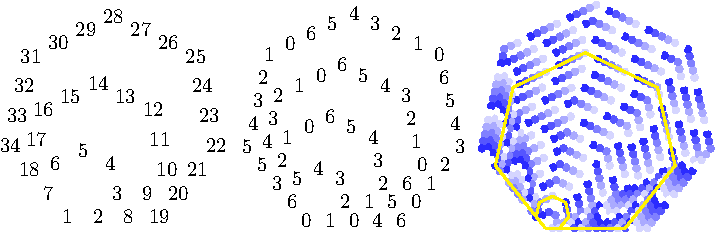
\includegraphics{Poly.pdf}
  % \centering
  % \begin{minipage}{0.3\linewidth}
  %   \input pics/Poly-1
  % \end{minipage}
  % \quad
  % \begin{minipage}{0.3\linewidth}
  %   \input pics/Poly-2
  % \end{minipage}
  % \quad
  % \begin{minipage}{0.3\linewidth}
  %   \input pics/Poly-3
  % \end{minipage}
  \caption{Polygonal numbers $P^7_m$ with $s=7$ sides: enumerated,
    counted $\pmod 7$ and shaded $\pmod 6$.}
  \label{fig:poly}
\end{figure}

We could generate such a nonlinear function $F$ by considering more
complicated tilings, which would then make our spirals much less
regular, and indeed we may have to reconsider what we mean by a
complete spiral in that case.  Alternatively, we could drop the
insistence that the spirals fill in each point of the lattice, which
would yield a generalization to polygonal numbers \cite{Polyg}.  These numbers
count the number of dots used in forming regular polygons, in which
the polygons are formed with one vertex at the origin, and each side
uses an integer number of dots (with vertices counted twice and some
dots reused), as illustrated in Figure~\ref{fig:poly}.  These generate
the polygonal numbers $P^s_m$, where $s$ is the number of sides in
the polygon, and $m$ is the number of dots per edge.  The first
polygonal number for $s$ sides is 1, so $P^s_1=1$, and the second is
the number of edges or vertices, $P^s_2=s$.  In general, the
polygonal numbers are given by
\[
  P^s_m = \frac{m(2+(s-2)(m-1))}2.
\]
For $s=3$ and $s=4$, these match the triangular numbers and squares;
generation of these leaves no gaps between dots and they fill a
regular lattice.

\begin{figure}[htb]
  \centering
  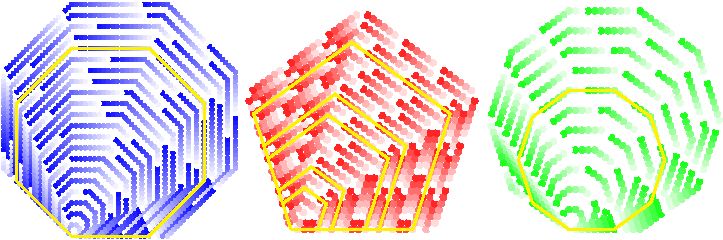
\includegraphics{Poly2.pdf}
  % 
  % \begin{minipage}{0.3\linewidth}
  %   \input pics/Poly8-18
  % \end{minipage}
  % \quad
  % \begin{minipage}{0.3\linewidth}
  %   \input pics/Poly5-7
  % \end{minipage}
  % \quad
  % \begin{minipage}{0.3\linewidth}
  %   \input pics/Poly10-8
  % \end{minipage}
  \caption{Grayscale counting: $P^8\pmod{18}$, $P^5\pmod7$ and $P^{10}\pmod8$.}
  \label{fig:poly2}
\end{figure}

A sample of generated figures is shown in Figure~\ref{fig:poly2}, for
varying number of sides $s$ and varying count $n$.  In particular, a
regular pattern such as that seen in the third picture $P^{10}\pmod8$,
is seen whenever $n=s-2$.  Although we enumerate these polygons in a
methodical way, we do not spiral out, which clearly shows in the
patterns generated by grayscale visualization.  However, we can still
define a complete $Ond_n$ pattern and test it by the condition $n\mid
P^s_m$.  By way of example, the hexagonal numbers are defined as
\[
	H_m = P^6_m = m\,(2m - 1),
\]
and we consider the condition $n \vert H_m$.  First, since $2m-1$ is
always odd, it follows that $m$ must be even whenever $n$ is.  Also,
any $Ond_n$ is achievable by taking $m$ a multiple of $n$.  Similarly,
if $n$ is prime, then we get complete $Ond_n$ patterns only if $m$ or
$2m-1$ is a multiple of $n$.  Thus, for example, taking $n=11$, we see
that the hexagons
\[
H_{6}, H_{11}, H_{17}, H_{22}, H_{28}, \ldots
\]
are achievable; the pattern is $m = 6 \xrightarrow{+5} 11
\xrightarrow{+6} 17 \xrightarrow{+5} 22 \xrightarrow{+6} \ldots$.
Similar alternating patterns are found for $Ond_{10}$, which has $m =
8 \xrightarrow{+2} 10 \xrightarrow{+8} 18 \xrightarrow{+2} 20
\xrightarrow{+8} 28 \xrightarrow{+2} \ldots$.  Note that the sum of
consecutive differences is the value of $n$ in both of these cases.
For $n = 15$, the pattern is over more than two values: $m = 18
\xrightarrow{+2} 20 \xrightarrow{+3} 23 \xrightarrow{+7} 30
\xrightarrow{+3} 33 \xrightarrow{+2} \ldots$. The pattern repeats and
the sum over the $m$ differences is again 15.  In the case of $n = 16
= 2^4$, we must have $16\mid m$, and the difference between successive
$m$ values is 16.  Indeed, since multiples of $n$ always yield
complete patterns, sums of appropriately chosen consecutive
differences will always be $n$, whether or not these patterns repeat.

\subsection*{Other Questions:}

There are several related ways to build up similar patterns starting
from the elementary spirals developed here, with different levels of
complexity.  Some possibilities are:
\begin{itemize}
\item Investigate non-square shapes in higher dimensions $d > 2$.
\item Investigate random $Ond$:
\begin{enumerate}
\item Select $n_1$ randomly, generate one or more complete $Ond_{n_1}$
  spirals; 
\item Select $n_2$ randomly, and continue spiraling until completing
  some subsequent $Ond_{n_2}$ spiral;
\item Repeat this process, with any number of $n_j$ spirals.
\end{enumerate}
\item Generate spirals of spirals: that is, form a given complete
  spiral, say $Ond_n^k$.  Now, use this as a block and generate
  ``block spirals'' out of the original $Ond_n^k$.
\end{itemize}

\subsection*{Remarks on picture generation:}

The authors have developed several programs for generation and
visualization of spirals, implemented in the python programming
language.  In all cases, the key step is to generate an array of
coordinates for the cells, corresponding to our enumeration $\ell_j$
of the spiral.  Once this is accomplished, it is not difficult to
count the spiral in any $\ZZ_n$, or indeed to assign a grayscale (or
color) value to the corresponding cell.

Our initial program generated spirals in which each cell was
represented by a single pixel; while this is not very practical for
small spirals, it can be used to generate many large spirals.
Grayscale images were generated for many square, triangular and
hexagonal $Ond_n^k$ spirals, and these are available at {\tt
 https://github.com/OndGen/gray}.  We have also generated a video visualization
showing changes in the spirals as the parameters change.  Next, we
implemented a code which allowed us to control the shape of the cells
as in Fig.~\ref{fig:trishades}.  We then implemented a GUI interface,
which allows interactive setting of parameters and generation of
spirals \cite{spyrrals}.  A small modification allowed us to generate the polygonal
patterns.  We are currently developing a web-based application, and we
expect to eventually implement it as a freely available stand-alone
cellphone app.

All of these and some related programs are freely available at {\tt
  https://github.com/OndGen} under the GPL/copyleft.  Our hope is that
availability of an easy-to-use app will allow teachers and other
interested parties to encourage students to experiment with these
spirals, find patterns and make conjectures, in an attempt to inspire
students to remain actively engaged in mathematical pursuits.



\begin{acknowledgment}{Acknowledgment.}
  The first author recognizes Veracode Inc for providing support and
  Jared Carlson of Veracode Research for fruitful discussion.  The
  second thanks his colleague Paul Gunnells for providing the proof of
  the ``only if'' part of Conjecture 1.
\end{acknowledgment}

\begin{thebibliography}{1}
\bibitem{PySquare} Young, R., Reiter, A., \url{https://github.com/OndGen/gray/code}
\bibitem{spyrrals} ---, \url{https://github.com/OndGen/spyrrals/}
\bibitem{OEIS} The On-Line Encyclopedia of Integer Sequences, \url{http://www.oeis.org/}
\bibitem{Davenport} Davenport, H., ``The Higher Arithmetic: An Introduction to the Theory of Numbers'', Cambridge, England: Cambridge University Press
\bibitem{Polyg} Weisstein, Eric W., ``Polygonal Number.'' From MathWorld--A Wolfram Web Resource. \url{http://mathworld.wolfram.com/PolygonalNumber.html} 
\bibitem{Ulam} --- ``Prime Spiral.'' From MathWorld--A Wolfram Web Resource. \url{http://mathworld.wolfram.com/PrimeSpiral.html}
\end{thebibliography}

\begin{biog}
\item[Andrew Reiter]  received his M.S. in
  applied mathematics from the University of Massachusetts-Amherst. He
  currently works as a computer security researcher for Veracode,
  Inc., a Boston based application security company.
\begin{affil}
Research,  Veracode, Inc., 65 Network Drive, Burlington MA 01803\\
areiter@veracode.com
\end{affil}

\item[Robin Young] studies nonlinear waves and their interactions in
  hyperbolic systems of conservation laws, particularly the equations
  of fluid dynamics and classical mechanics.  He is a Professor in the
  Department of Mathematics \& Statistics at the University of
  Massachusetts-Amherst and received his Ph.D. from University of
  California-Davis.
\begin{affil}
Department of Mathematics \& Statistics, UMASS-Amherst, Amherst MA 01003 \\
young@math.umass.edu
\end{affil}
\end{biog}
\vfill\eject

\end{document}
